\mbox{}\\
\vspace{8cm}

This chapter is a reproduction of the following submitted manuscript for publication in GigaScience:

C. I. Mendes, P. Vila-Cerqueira, Y. Motro, J. Moran-Gilad, J. A. Carriço, M. Ramirez. LMAS: Last Metagenomic Assembler Standing

The supplementary information referred throughout the text can be consulted in this chapter before the section of references.

Short-read \ac{SMg} can offer comprehensive microbial detection and characterisation of complex clinical samples. The \textit{de novo} assembly of raw sequence data is key in metagenomic analysis, yielding longer sequences that offer contextual information and afford a more complete picture of the microbial community. The assembly process is the bedrock and may constitute a major bottleneck in obtaining trustworthy, reproducible results.

In this chapter, we present LMAS, an automated workflow developed as a flexible platform to allow users to evaluate traditional and metagenomic dedicated prokaryotic de novo assembly software performance given known standard communities. Its implementation in Nextflow ensures the transparency and reproducibility of the results obtained and the use of Docker containers provides further flexibility. The results are presented in an interactive HTML report where global and reference specific performance metrics can be explored. Currently, 12 assemblers still being maintained are implemented in LMAS, with the possibility of expansion as novel algorithms are developed.

To showcase LMAS we used a test dataset of eight bacterial genomes and four plasmids of the ZymoBIOMICS Microbial Community Standards with linear and logarithmic distribution,  and found that k-mer De Bruijn graph assemblers outperformed the alternative approaches but came with a greater computational cost. Furthermore, assemblers branded as metagenomic specific did not consistently outperform other genomic assemblers in metagenomic samples. Some assemblers still in use, such as ABySS, BCALM2, MetaHipmer2, minia and VelvetOptimiser,  showed significant performance problems and their usability may be limited, particularly when assembling complex samples. 

The performance of each assembler varied depending on the species of interest and its abundance in the sample, with less abundant species presenting a significant challenge for all assemblers. No assembler stood out as an undisputed all-purpose choice for short-read metagenomic prokaryote genome assembly, highlighting that efforts are still needed to further improve metagenomic assembly performance. Our results also suggest that sample complexity and a particular interest in some sample components may affect assembler choice. Using LMAS could help users in their choice of assembler for their specific purpose.  As such, we believe that this manuscript is appropriate for publication in Microbiome as a Software article. 

My contribution to this publication included the design, implementation and optimisation of the LMAS the workflow, including the creation of the Docker containers for all dependencies. I performed the data analysis and comparison of assemblers included in LMAS with ZymoBIOMICS Microbial Community Standards, both evenly and logarithmically distributed samples. Additionally, I've also wrote the manuscript.

\cleardoublepage 

\begin{center}
\large
\textbf{LMAS: Last Metagenomic Assembler Standing}
\end{center}

Catarina I Mendes$^1,*$, 
P Vila-Cerqueira$^1*$,
Y Motro$^2$,
J. Moran-Gilad$^2$,
João A Carriço$^1$
Mário Ramirez$^1$, 


$^1$Instituto de Microbiologia, Instituto de Medicina Molecular, Faculdade de Medicina, Universidade de Lisboa, Lisboa, Portugal 

$^2$Faculty of Health Sciences, Ben-Gurion University of the Negev, Beer-Sheva, Israel

\section{Abstract}

\textbf{Background }The de novo assembly of raw sequence data is key in metagenomic analysis. It allows recovering draft genomes from a pool of mixed raw reads, yielding longer sequences that offer contextual information and provide a more complete picture of the microbial community.
\textbf{Results} To better compare de novo assemblers for metagenomic analysis, LMAS was developed as a flexible platform allowing users to evaluate assembler performance given known standard communities. Overall, in our test datasets, k-mer De Bruijn graph assemblers outperformed the alternative approaches but came with a greater computational cost. Furthermore, assemblers branded as metagenomic specific did not consistently outperform other genomic assemblers in metagenomic samples. Some assemblers still in use, such as ABySS, BCALM2, MetaHipmer2, minia and VelvetOptimiser, perform relatively poorly and should be used with caution when assembling complex samples. 
\textbf{Conclusions} The choice of a de novo assembler depends on the computational resources available, the replicon of interest, and the major goals of the analysis. No single assembler appeared an ideal choice for short-read metagenomic prokaryote replicon assembly, each showing specific strengths. The choice of metagenomic assembler should be guided by user requirements and characteristics of the sample of interest, and LMAS provides an interactive evaluation platform for this purpose. 

\subsubsection{Keywords}

Shotgun Metagenomics, de novo assembly, benchmark, draft genome quality, simulation

\section{Background}

Short-read shotgun metagenomics has the potential to offer comprehensive microbial detection and characterisation of complex clinical or environmental samples.  Despite becoming an increasingly used approach, it comes at the cost of producing massive amounts of data that require expert handling and processing, as well as adequate computational resources. The de novo assembly process is key when analysing metagenomic data since it allows recovering contigs representing the replicons present in the sample, be it genomes, plasmids or bacteriophages, from a pool of mixed raw reads. These contigs are longer sequences that offer better contextual information than reads alone and provide a more complete picture of the microbial community than the species composition. Despite efforts for the development, standardisation and assessment of software for metagenomic analysis, both commercial and open-source \cite{angers-loustau_challenges_2018,gruening_recommendations_2019, sczyrba_critical_2017, couto_critical_2018, meyer_critical_2021}, the de novo assembly process still represents a critical point in these analyses.

The assembly of draft genomes has become a central step when analysing pure bacterial cultures, for instance allowing genomic comparisons through single nucleotide \ac{SNP}s or gene-by-gene methods, such as \ac{cgMLST}. The first assemblers implemented \ac{OLC} approaches, comparing all reads in a sample, computing overlaps and generating consensus sequences by picking the most likely nucleotide for each position in the contigs. As the throughput of sequencing methods increased exponentially, so did the number of pairwise comparisons, limiting the efficiency of these algorithms and making them computationally too expensive. To circumvent this, \ac{dBg} algorithms were increasingly adopted and are currently the most widely used approaches in modern assembly software. Both \ac{OLC} and \ac{dBg} handle unresolvable repeats by essentially fragmenting the sequence, that is, forming multiple contigs for each of the possibly contiguous sequences present in the sample. Additionally, the inherent heterogeneity of complex samples, potentially containing a multitude of replicons, could make traditional genome assemblers, implementing optimisations based on the assumption of having a single genome in the sample, not suitable for metagenomics \cite{ayling_new_2020}.

Several dedicated metagenomic assembly tools for short-read data are available \cite{ayling_new_2020}. These tools are generally assumed to perform better when dealing with complex samples having a combination of intragenomic and intergenomic repeats and uneven and low coverage sequencing depths of some of the replicons \cite{olson_metagenomic_2019}. Not using dedicated metagenomic assemblers was suggested to come with the cost of generating artificial variation and chimeric contigs, especially in samples that contain closely related species \cite{teeling_current_2012}. However, to our knowledge, no formal comparison has been done looking at increased accuracy or gains in contiguity of assemblies obtained with metagenomic assemblers versus traditional assemblers.

With an ever-increasing range of both traditional and metagenomic assemblers becoming available, choosing the best performing tool can be an arduous and time-consuming task since the choice may vary depending on the purpose of the analysis, organism of interest, complexity of the sample and computational infrastructure available. Additionally, the evaluation of the resulting contigs is not straightforward since one metric is not sufficient to classify an assembly, particularly with complex samples \cite{olson_metagenomic_2019,bradnam_assemblathon_2013}. Despite several de novo assembly validation methods relying on features of the created contigs themselves, such as QUAST \cite{gurevich_quast_2013}, being useful in identifying inconsistencies indicative of potential assembly errors, the use of reference-based validation methods offer the possibility of a more complete evaluation of accuracy and are particularly important to benchmark attempts to reconstruct communities. MetaQUAST \cite{bradnam_assemblathon_2013}, a modification of QUAST, extends the original software by performing assembly evaluation based on aligning contigs to a reference, which can be provided or inferred by the software, and reports, in addition to the standard metrics for single genomes reported by QUAST, the number of interspecies translocations and the number of possibly misassembled contigs.

The use of mock communities, with known composition, abundance and genomic information, provides a ground truth against which the success of the assembly of a complex sample can be evaluated. Such mock communities facilitate the identification of misassemblies, such as chimeric sequences generated from the improper combination of two distinct replicons, indels or single nucleotide variants improperly created by the assembler. On the other hand, the comparison of the performance of two assemblers is only possible if the input data is the same and if the same evaluation metrics are applied \cite{sczyrba_critical_2017}. 

To tackle these challenges, we developed LMAS (Last Metagenomic Assembler Standing), an automated workflow to enable the benchmarking of traditional and metagenomic prokaryotic de novo assembly software using defined mock communities. The results of LMAS are presented in an interactive HTML report where selected global and reference replicon specific performance metrics can be explored. The mock communities can be provided by the user to better reflect the samples of interest. New assemblers can be added with minimal changes to the pipeline so that LMAS can be expanded to include novel algorithms as they are developed. The portability and ease of use of LMAS is intended to allow users to evaluate the performance of assemblers in mock communities, mimicking as closely as possible their samples of interest. LMAS is open source and the workflow and its documentation are available at \url{https://github.com/B-UMMI/LMAS} and \url{https://lmas.readthedocs.io/} respectively. 

\subsection{Implementation}

\subsubsection{Workflow overview}

LMAS is a user-friendly automated workflow enabling the benchmarking of traditional and metagenomic prokaryotic de novo assembly software using defined mock communities. LMAS was implemented in Nextflow [12]\cite{di_tommaso_nextflow_2017} to provide flexibility and ensure the transparency and reproducibility of the results. LMAS relies on the use of Docker \cite{merkel_docker_2014} containers for each assembler, allowing versions to be tracked and changed easily.

\begin{figure*}[h!]
\centering
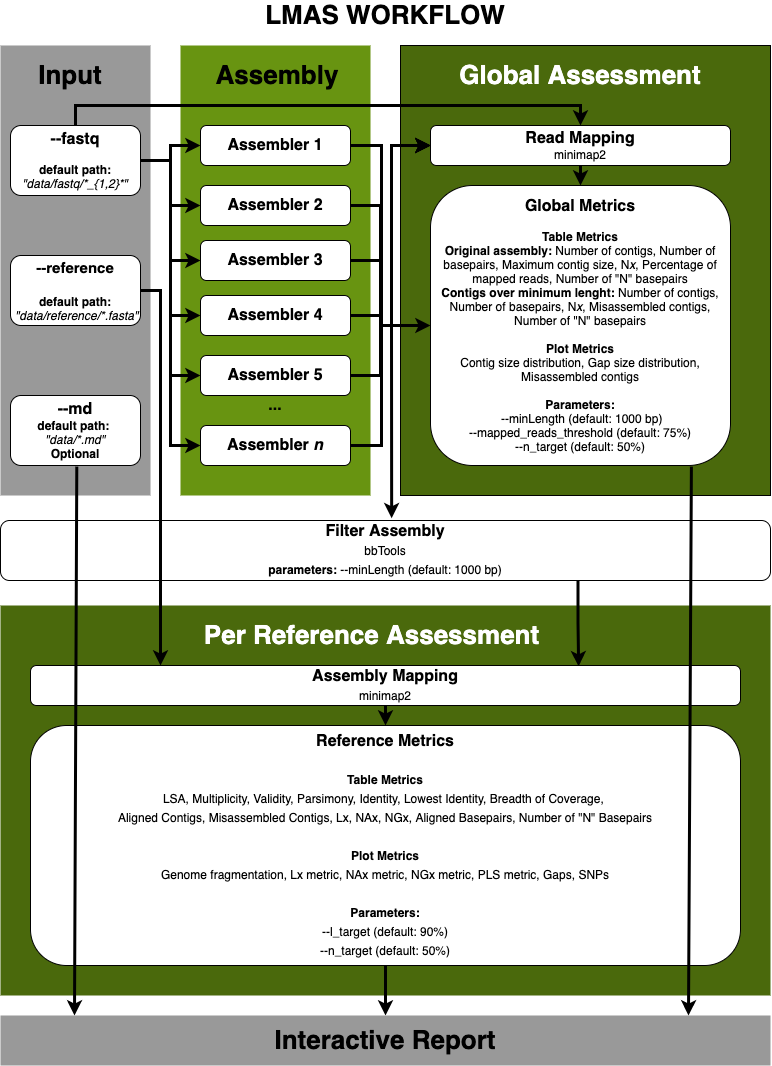
\includegraphics[width=\textwidth]{figures/chapter 5/Figure 1.png}
\caption{The LMAS workflow. The input sequencing data is assembled in parallel, resources permitting, by the set of assemblers included in LMAS. The resulting contigs are processed and the global quality assessment is performed. After filtering for the user-defined minimum contig size, the remaining sequences are mapped against the provided reference and the resulting information is processed to evaluate assembly quality by replicon in the reference file. All results, and optional text information describing the samples, are grouped in the LMAS report.}
\label{fig:chap5_figure1}
\end{figure*}

\subsubsection{Installation and Usage}

LMAS can be installed through Bioconda \cite{noauthor_lmas_2021} or Github \cite{mendes_lmas_2021}, with detailed instructions available in the documentation \cite{noauthor_installation_nodate}. LMAS requires as inputs the complete reference replicons (genomes, plasmids or any other replicons present) and short-read paired-end raw data. All complete references (linear replicons) should be provided in a single file. This raw data can be either obtained in silico by creating simulated reads from the reference replicons or sequencing mock communities of known composition. Optionally, information on the input samples in a markdown file can be provided to be presented in the report.

A step-by-step execution tutorial is available at \cite{noauthor_basic_nodate}. Users can customise the workflow execution either by using command-line options or by modifying the simple plain-text configuration files. To make the execution of the workflow as simple as possible, a set of default parameters and directives is provided. A complete description of each parameter is available in Supplemental Material (see Supplemental Material, Workflow parameters), as well as in the documentation \cite{noauthor_parameters_nodate}.  The results are presented in an interactive HTML report, stored in the “report” folder in the directory of LMAS’ execution. The output files of all assemblers and quality assessment processing scripts in the workflow are stored in the “results” folder, in the same location. 